\documentclass[twoside]{book}

% Packages required by doxygen
\usepackage{fixltx2e}
\usepackage{calc}
\usepackage{doxygen}
\usepackage[export]{adjustbox} % also loads graphicx
\usepackage{graphicx}
\usepackage[utf8]{inputenc}
\usepackage{makeidx}
\usepackage{multicol}
\usepackage{multirow}
\PassOptionsToPackage{warn}{textcomp}
\usepackage{textcomp}
\usepackage[nointegrals]{wasysym}
\usepackage[table]{xcolor}

% Font selection
\usepackage[T1]{fontenc}
\usepackage[scaled=.90]{helvet}
\usepackage{courier}
\usepackage{amssymb}
\usepackage{sectsty}
\renewcommand{\familydefault}{\sfdefault}
\allsectionsfont{%
  \fontseries{bc}\selectfont%
  \color{darkgray}%
}
\renewcommand{\DoxyLabelFont}{%
  \fontseries{bc}\selectfont%
  \color{darkgray}%
}
\newcommand{\+}{\discretionary{\mbox{\scriptsize$\hookleftarrow$}}{}{}}

% Page & text layout
\usepackage{geometry}
\geometry{%
  a4paper,%
  top=2.5cm,%
  bottom=2.5cm,%
  left=2.5cm,%
  right=2.5cm%
}
\tolerance=750
\hfuzz=15pt
\hbadness=750
\setlength{\emergencystretch}{15pt}
\setlength{\parindent}{0cm}
\setlength{\parskip}{3ex plus 2ex minus 2ex}
\makeatletter
\renewcommand{\paragraph}{%
  \@startsection{paragraph}{4}{0ex}{-1.0ex}{1.0ex}{%
    \normalfont\normalsize\bfseries\SS@parafont%
  }%
}
\renewcommand{\subparagraph}{%
  \@startsection{subparagraph}{5}{0ex}{-1.0ex}{1.0ex}{%
    \normalfont\normalsize\bfseries\SS@subparafont%
  }%
}
\makeatother

% Headers & footers
\usepackage{fancyhdr}
\pagestyle{fancyplain}
\fancyhead[LE]{\fancyplain{}{\bfseries\thepage}}
\fancyhead[CE]{\fancyplain{}{}}
\fancyhead[RE]{\fancyplain{}{\bfseries\leftmark}}
\fancyhead[LO]{\fancyplain{}{\bfseries\rightmark}}
\fancyhead[CO]{\fancyplain{}{}}
\fancyhead[RO]{\fancyplain{}{\bfseries\thepage}}
\fancyfoot[LE]{\fancyplain{}{}}
\fancyfoot[CE]{\fancyplain{}{}}
\fancyfoot[RE]{\fancyplain{}{\bfseries\scriptsize Generated by Doxygen }}
\fancyfoot[LO]{\fancyplain{}{\bfseries\scriptsize Generated by Doxygen }}
\fancyfoot[CO]{\fancyplain{}{}}
\fancyfoot[RO]{\fancyplain{}{}}
\renewcommand{\footrulewidth}{0.4pt}
\renewcommand{\chaptermark}[1]{%
  \markboth{#1}{}%
}
\renewcommand{\sectionmark}[1]{%
  \markright{\thesection\ #1}%
}

% Indices & bibliography
\usepackage{natbib}
\usepackage[titles]{tocloft}
\setcounter{tocdepth}{3}
\setcounter{secnumdepth}{5}
\makeindex

% Hyperlinks (required, but should be loaded last)
\usepackage{ifpdf}
\ifpdf
  \usepackage[pdftex,pagebackref=true]{hyperref}
\else
  \usepackage[ps2pdf,pagebackref=true]{hyperref}
\fi
\hypersetup{%
  colorlinks=true,%
  linkcolor=blue,%
  citecolor=blue,%
  unicode%
}

% Custom commands
\newcommand{\clearemptydoublepage}{%
  \newpage{\pagestyle{empty}\cleardoublepage}%
}

\usepackage{caption}
\captionsetup{labelsep=space,justification=centering,font={bf},singlelinecheck=off,skip=4pt,position=top}

%===== C O N T E N T S =====

\begin{document}

% Titlepage & ToC
\hypersetup{pageanchor=false,
             bookmarksnumbered=true,
             pdfencoding=unicode
            }
\pagenumbering{alph}
\begin{titlepage}
\vspace*{7cm}
\begin{center}%
{\Large Flocking\+Library \\[1ex]\large 0.\+1 }\\
\vspace*{1cm}
{\large Generated by Doxygen 1.8.13}\\
\end{center}
\end{titlepage}
\clearemptydoublepage
\pagenumbering{roman}
\tableofcontents
\clearemptydoublepage
\pagenumbering{arabic}
\hypersetup{pageanchor=true}

%--- Begin generated contents ---
\chapter{P\+S\+Flocking\+Library}
\label{index}\hypertarget{index}{}\hypertarget{index_intro_sec}{}\section{Introduction}\label{index_intro_sec}
P\+S\+Flocking\+Library is a customizable Unity3D Flocking-\/\+Library used on Rigidbodies. It follows three general rules\+: 1) Alignment 2) Cohesion 3) Separation 4) Optional\+: Follow a \char`\"{}goal\char`\"{}-\/\+Game\+Object

Each of these rules can be overriden to calculate a custom force that should be added to the boid, providing a lot of flexibility.\hypertarget{index_install_sec}{}\section{Installation}\label{index_install_sec}
You can download the complete Sourcecode with a unity project containing two example scenes demonstrating standard flocking, and a subclassed example. Alternatively you can download the .dll file on the Release page on Git\+Hub.

In your .cs files, add a \char`\"{}using P\+S\+Flocking;\char`\"{} statement. In Unity, add the P\+S\+Unit\+Manager to a gameobject, and set its variables in the inspector. Important\+: Set at least the \char`\"{}\+Unit Prefab\char`\"{} variable. If you want to use a goal that the units should follow, then also set the \char`\"{}\+Goal\char`\"{} variable. Change the other parameters as you like to get a feeling for them.

You can add and remove units at any time by calling Add\+Flocking\+Unit and Remove\+Flocking\+Unit on the P\+S\+Unit\+Manager script.\hypertarget{index_usage_sec}{}\section{Usage}\label{index_usage_sec}
The four functions Alignment, Cohesion, Separation and Seek\+Goal can be subclassed. Each of them returns a Vector3 representing a force that will be applied on the unit\textquotesingle{}s rigidbody. All four forces will be added together, normalized, and then applied to the rigidbody. By subclassing P\+S\+Flocking\+Unit, you can implement custom versions of these 4 functions. Take a look at the P\+S\+Flocking\+Unit class for further details on the functions. 
\chapter{Namespace Index}
\section{Packages}
Here are the packages with brief descriptions (if available)\+:\begin{DoxyCompactList}
\item\contentsline{section}{\hyperlink{namespace_p_s_flocking}{P\+S\+Flocking} }{\pageref{namespace_p_s_flocking}}{}
\end{DoxyCompactList}

\chapter{Hierarchical Index}
\section{Class Hierarchy}
This inheritance list is sorted roughly, but not completely, alphabetically\+:\begin{DoxyCompactList}
\item Mono\+Behaviour\begin{DoxyCompactList}
\item \contentsline{section}{F\+Flocking\+Unit}{\pageref{class_f_flocking_unit}}{}
\item \contentsline{section}{F\+Goal\+Random\+Movement}{\pageref{class_f_goal_random_movement}}{}
\item \contentsline{section}{F\+Unit\+Manager}{\pageref{class_f_unit_manager}}{}
\item \contentsline{section}{Unit\+Manager}{\pageref{class_unit_manager}}{}
\end{DoxyCompactList}
\end{DoxyCompactList}

\chapter{Class Index}
\section{Class List}
Here are the classes, structs, unions and interfaces with brief descriptions\+:\begin{DoxyCompactList}
\item\contentsline{section}{\hyperlink{class_f_flocking_unit}{F\+Flocking\+Unit} }{\pageref{class_f_flocking_unit}}{}
\item\contentsline{section}{\hyperlink{class_f_goal_random_movement}{F\+Goal\+Random\+Movement} }{\pageref{class_f_goal_random_movement}}{}
\item\contentsline{section}{\hyperlink{class_f_unit_manager}{F\+Unit\+Manager} }{\pageref{class_f_unit_manager}}{}
\item\contentsline{section}{\hyperlink{class_unit_manager}{Unit\+Manager} }{\pageref{class_unit_manager}}{}
\end{DoxyCompactList}

\chapter{Namespace Documentation}
\hypertarget{namespace_p_s_flocking}{}\section{P\+S\+Flocking Namespace Reference}
\label{namespace_p_s_flocking}\index{P\+S\+Flocking@{P\+S\+Flocking}}
\subsection*{Classes}
\begin{DoxyCompactItemize}
\item 
class \hyperlink{class_p_s_flocking_1_1_p_s_flocking_unit}{P\+S\+Flocking\+Unit}
\item 
class \hyperlink{class_p_s_flocking_1_1_p_s_unit_manager}{P\+S\+Unit\+Manager}
\end{DoxyCompactItemize}

\chapter{Class Documentation}
\hypertarget{class_p_s_camera_manager}{}\section{P\+S\+Camera\+Manager Class Reference}
\label{class_p_s_camera_manager}\index{P\+S\+Camera\+Manager@{P\+S\+Camera\+Manager}}
Inheritance diagram for P\+S\+Camera\+Manager\+:\begin{figure}[H]
\begin{center}
\leavevmode
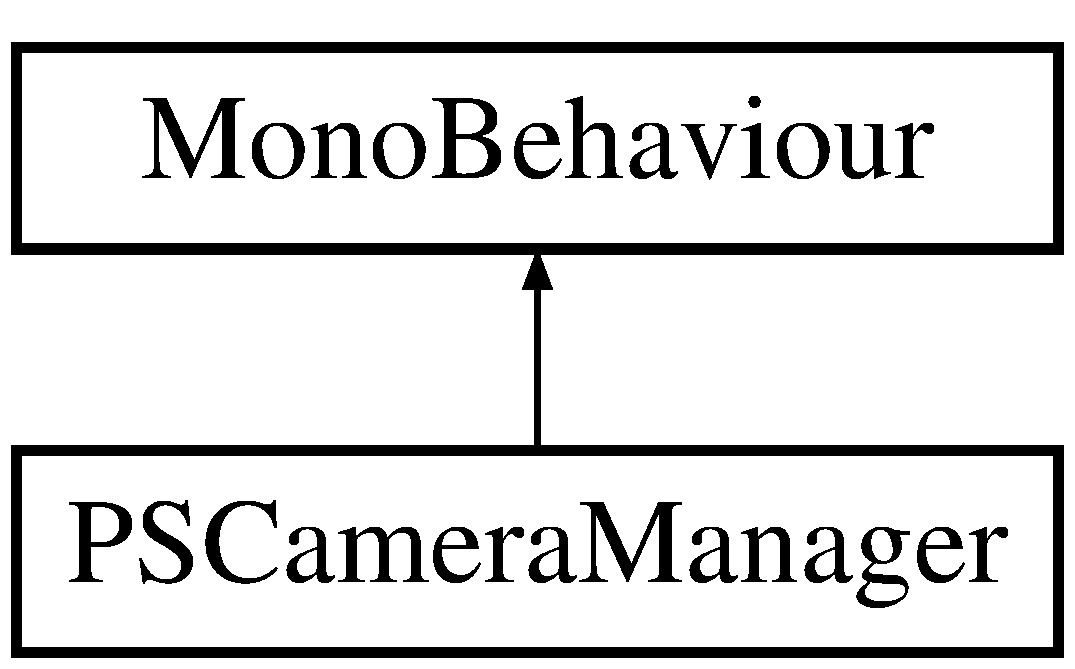
\includegraphics[height=2.000000cm]{class_p_s_camera_manager}
\end{center}
\end{figure}


The documentation for this class was generated from the following file\+:\begin{DoxyCompactItemize}
\item 
Assets/\+\_\+\+Scripts/P\+S\+Camera\+Manager.\+cs\end{DoxyCompactItemize}

\hypertarget{class_p_s_custom_flocker}{}\section{P\+S\+Custom\+Flocker Class Reference}
\label{class_p_s_custom_flocker}\index{P\+S\+Custom\+Flocker@{P\+S\+Custom\+Flocker}}
Inheritance diagram for P\+S\+Custom\+Flocker\+:\begin{figure}[H]
\begin{center}
\leavevmode
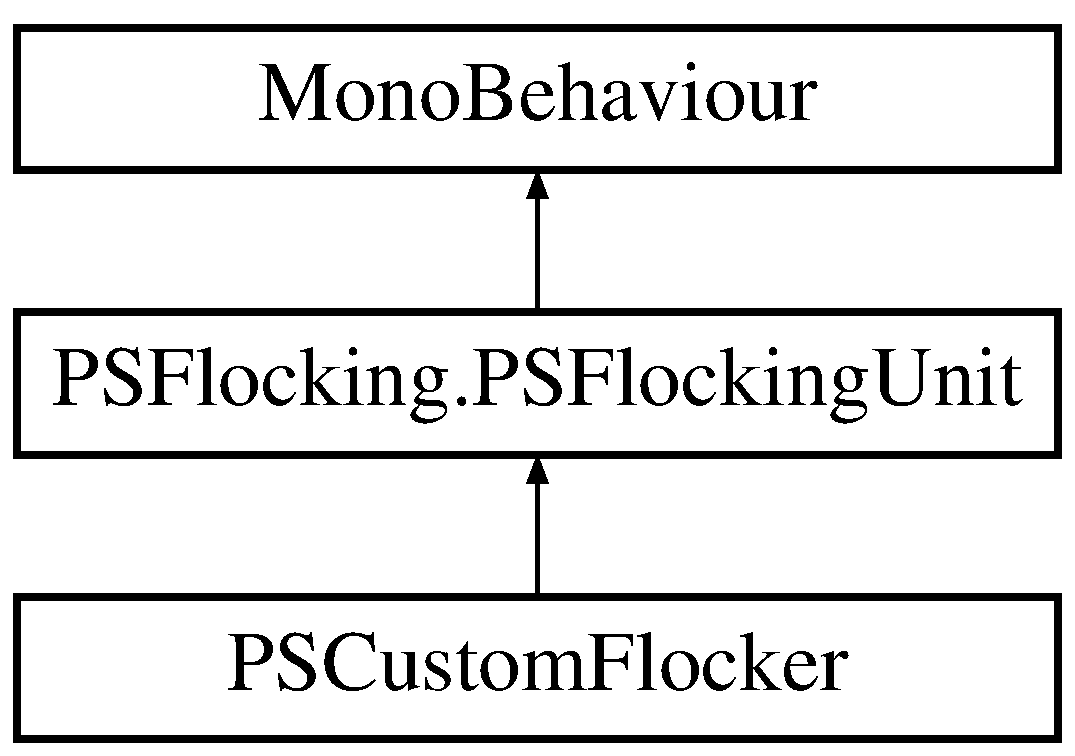
\includegraphics[height=3.000000cm]{class_p_s_custom_flocker}
\end{center}
\end{figure}
\subsection*{Public Member Functions}
\begin{DoxyCompactItemize}
\item 
\hyperlink{class_p_s_custom_flocker_aecf3471651ecc3e957b5144b0e6b9b21}{P\+S\+Custom\+Flocker} ()
\end{DoxyCompactItemize}
\subsection*{Protected Member Functions}
\begin{DoxyCompactItemize}
\item 
override Vector3 \hyperlink{class_p_s_custom_flocker_a50d8ac4146196420bcf1181289a27e40}{Align} ()
\begin{DoxyCompactList}\small\item\em Align function, overridden from P\+S\+Flocking\+Unit. \end{DoxyCompactList}\item 
override Vector3 \hyperlink{class_p_s_custom_flocker_a46d7ff69872c12983a666293794b976f}{Cohesion} ()
\begin{DoxyCompactList}\small\item\em Cohesion function, overridden from P\+S\+Flocking\+Unit. \end{DoxyCompactList}\item 
override Vector3 \hyperlink{class_p_s_custom_flocker_a2ab0990e603a5102fc80dafee1333c7c}{Separation} ()
\begin{DoxyCompactList}\small\item\em Separation function, overridden from P\+S\+Flocking\+Unit. \end{DoxyCompactList}\item 
override Vector3 \hyperlink{class_p_s_custom_flocker_a43590dd2fdf5f37d2116cf08473375c7}{Seek\+Goal} ()
\begin{DoxyCompactList}\small\item\em Seek\+Goal function, overridden from P\+S\+Flocking\+Unit. \end{DoxyCompactList}\end{DoxyCompactItemize}
\subsection*{Additional Inherited Members}


\subsection{Constructor \& Destructor Documentation}
\mbox{\Hypertarget{class_p_s_custom_flocker_aecf3471651ecc3e957b5144b0e6b9b21}\label{class_p_s_custom_flocker_aecf3471651ecc3e957b5144b0e6b9b21}} 
\index{P\+S\+Custom\+Flocker@{P\+S\+Custom\+Flocker}!P\+S\+Custom\+Flocker@{P\+S\+Custom\+Flocker}}
\index{P\+S\+Custom\+Flocker@{P\+S\+Custom\+Flocker}!P\+S\+Custom\+Flocker@{P\+S\+Custom\+Flocker}}
\subsubsection{\texorpdfstring{P\+S\+Custom\+Flocker()}{PSCustomFlocker()}}
{\footnotesize\ttfamily P\+S\+Custom\+Flocker.\+P\+S\+Custom\+Flocker (\begin{DoxyParamCaption}{ }\end{DoxyParamCaption})}

An example class that implements custom movement. It is very primitive -\/ it moves the unit along the x-\/axis. 

\subsection{Member Function Documentation}
\mbox{\Hypertarget{class_p_s_custom_flocker_a50d8ac4146196420bcf1181289a27e40}\label{class_p_s_custom_flocker_a50d8ac4146196420bcf1181289a27e40}} 
\index{P\+S\+Custom\+Flocker@{P\+S\+Custom\+Flocker}!Align@{Align}}
\index{Align@{Align}!P\+S\+Custom\+Flocker@{P\+S\+Custom\+Flocker}}
\subsubsection{\texorpdfstring{Align()}{Align()}}
{\footnotesize\ttfamily override Vector3 P\+S\+Custom\+Flocker.\+Align (\begin{DoxyParamCaption}{ }\end{DoxyParamCaption})\hspace{0.3cm}{\ttfamily [protected]}, {\ttfamily [virtual]}}



Align function, overridden from P\+S\+Flocking\+Unit. 

\begin{DoxyReturn}{Returns}
Vector3 Alignment for the Unit, will be applied as a force on its rigidbody. 
\end{DoxyReturn}


Reimplemented from \hyperlink{class_p_s_flocking_1_1_p_s_flocking_unit_ada3fa9e23f12a1b8258dc324f5b3e511}{P\+S\+Flocking.\+P\+S\+Flocking\+Unit}.

\mbox{\Hypertarget{class_p_s_custom_flocker_a46d7ff69872c12983a666293794b976f}\label{class_p_s_custom_flocker_a46d7ff69872c12983a666293794b976f}} 
\index{P\+S\+Custom\+Flocker@{P\+S\+Custom\+Flocker}!Cohesion@{Cohesion}}
\index{Cohesion@{Cohesion}!P\+S\+Custom\+Flocker@{P\+S\+Custom\+Flocker}}
\subsubsection{\texorpdfstring{Cohesion()}{Cohesion()}}
{\footnotesize\ttfamily override Vector3 P\+S\+Custom\+Flocker.\+Cohesion (\begin{DoxyParamCaption}{ }\end{DoxyParamCaption})\hspace{0.3cm}{\ttfamily [protected]}, {\ttfamily [virtual]}}



Cohesion function, overridden from P\+S\+Flocking\+Unit. 

\begin{DoxyReturn}{Returns}
Vector3 Cohesion for the Unit, will be applied as a force on its rigidbody. 
\end{DoxyReturn}


Reimplemented from \hyperlink{class_p_s_flocking_1_1_p_s_flocking_unit_a87ad210603e8d8451e14a4de8af9cba0}{P\+S\+Flocking.\+P\+S\+Flocking\+Unit}.

\mbox{\Hypertarget{class_p_s_custom_flocker_a43590dd2fdf5f37d2116cf08473375c7}\label{class_p_s_custom_flocker_a43590dd2fdf5f37d2116cf08473375c7}} 
\index{P\+S\+Custom\+Flocker@{P\+S\+Custom\+Flocker}!Seek\+Goal@{Seek\+Goal}}
\index{Seek\+Goal@{Seek\+Goal}!P\+S\+Custom\+Flocker@{P\+S\+Custom\+Flocker}}
\subsubsection{\texorpdfstring{Seek\+Goal()}{SeekGoal()}}
{\footnotesize\ttfamily override Vector3 P\+S\+Custom\+Flocker.\+Seek\+Goal (\begin{DoxyParamCaption}{ }\end{DoxyParamCaption})\hspace{0.3cm}{\ttfamily [protected]}, {\ttfamily [virtual]}}



Seek\+Goal function, overridden from P\+S\+Flocking\+Unit. 

\begin{DoxyReturn}{Returns}
Vector3 Vector towards the goal Game\+Object of P\+S\+Unit\+Manager, or a zero-\/vector if that variable is not set. 
\end{DoxyReturn}


Reimplemented from \hyperlink{class_p_s_flocking_1_1_p_s_flocking_unit_ab2ce12145c79e5e179f841412ed2febb}{P\+S\+Flocking.\+P\+S\+Flocking\+Unit}.

\mbox{\Hypertarget{class_p_s_custom_flocker_a2ab0990e603a5102fc80dafee1333c7c}\label{class_p_s_custom_flocker_a2ab0990e603a5102fc80dafee1333c7c}} 
\index{P\+S\+Custom\+Flocker@{P\+S\+Custom\+Flocker}!Separation@{Separation}}
\index{Separation@{Separation}!P\+S\+Custom\+Flocker@{P\+S\+Custom\+Flocker}}
\subsubsection{\texorpdfstring{Separation()}{Separation()}}
{\footnotesize\ttfamily override Vector3 P\+S\+Custom\+Flocker.\+Separation (\begin{DoxyParamCaption}{ }\end{DoxyParamCaption})\hspace{0.3cm}{\ttfamily [protected]}, {\ttfamily [virtual]}}



Separation function, overridden from P\+S\+Flocking\+Unit. 

\begin{DoxyReturn}{Returns}
Vector3 Separation for the Unit, will be applied as a force on its rigidbody. 
\end{DoxyReturn}


Reimplemented from \hyperlink{class_p_s_flocking_1_1_p_s_flocking_unit_af486901d480a5520aeae135d46635e60}{P\+S\+Flocking.\+P\+S\+Flocking\+Unit}.



The documentation for this class was generated from the following file\+:\begin{DoxyCompactItemize}
\item 
Assets/\+\_\+\+Scripts/P\+S\+Custom\+Flocker.\+cs\end{DoxyCompactItemize}

\hypertarget{class_p_s_custom_flocking_example}{}\section{P\+S\+Custom\+Flocking\+Example Class Reference}
\label{class_p_s_custom_flocking_example}\index{P\+S\+Custom\+Flocking\+Example@{P\+S\+Custom\+Flocking\+Example}}
Inheritance diagram for P\+S\+Custom\+Flocking\+Example\+:\begin{figure}[H]
\begin{center}
\leavevmode
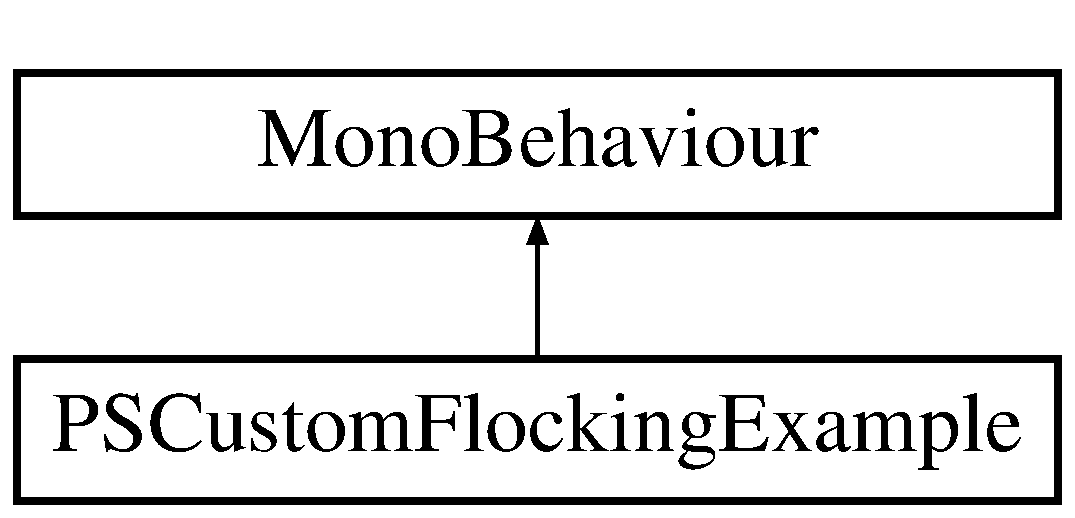
\includegraphics[height=2.000000cm]{class_p_s_custom_flocking_example}
\end{center}
\end{figure}
\subsection*{Public Attributes}
\begin{DoxyCompactItemize}
\item 
\mbox{\Hypertarget{class_p_s_custom_flocking_example_a2665ff1dc3ea0767286671e4f9a8a2cc}\label{class_p_s_custom_flocking_example_a2665ff1dc3ea0767286671e4f9a8a2cc}} 
Game\+Object {\bfseries manager}
\end{DoxyCompactItemize}


\subsection{Detailed Description}
An example class that adds custom units, with a custom flocking behaviour to the P\+S\+Unit\+Manager. 

The documentation for this class was generated from the following file\+:\begin{DoxyCompactItemize}
\item 
Assets/\+\_\+\+Scripts/P\+S\+Custom\+Flocking\+Example.\+cs\end{DoxyCompactItemize}

\hypertarget{class_p_s_flocking_1_1_p_s_flocking_unit}{}\section{P\+S\+Flocking.\+P\+S\+Flocking\+Unit Class Reference}
\label{class_p_s_flocking_1_1_p_s_flocking_unit}\index{P\+S\+Flocking.\+P\+S\+Flocking\+Unit@{P\+S\+Flocking.\+P\+S\+Flocking\+Unit}}
Inheritance diagram for P\+S\+Flocking.\+P\+S\+Flocking\+Unit\+:\begin{figure}[H]
\begin{center}
\leavevmode
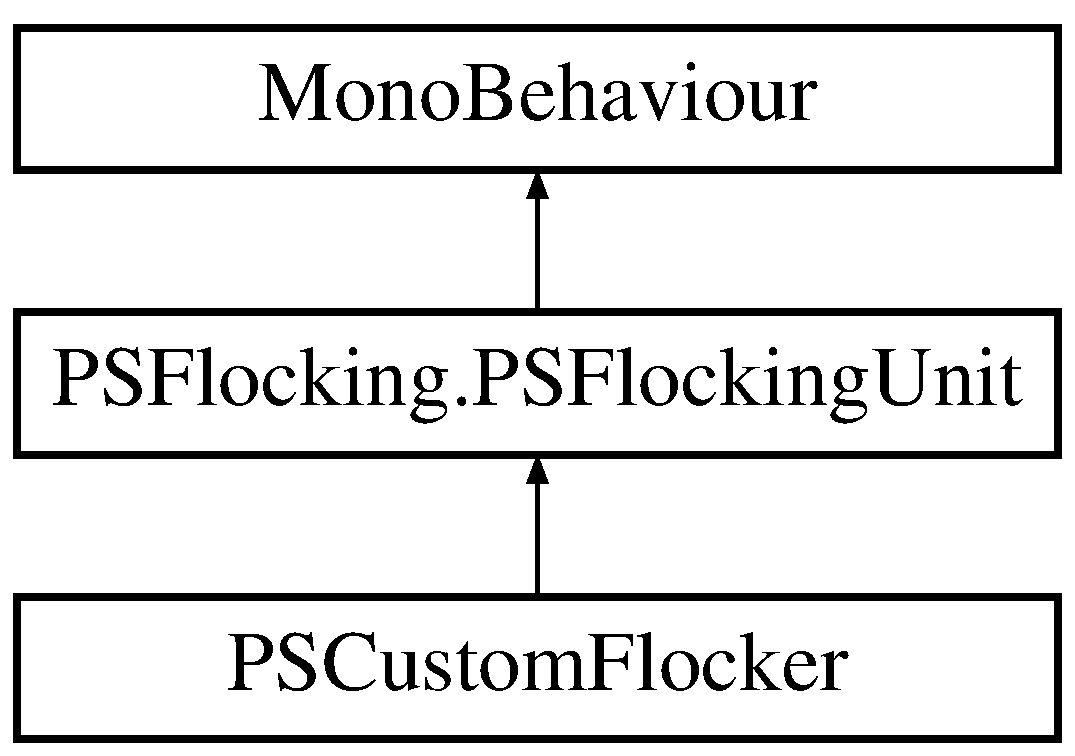
\includegraphics[height=3.000000cm]{class_p_s_flocking_1_1_p_s_flocking_unit}
\end{center}
\end{figure}
\subsection*{Protected Member Functions}
\begin{DoxyCompactItemize}
\item 
\mbox{\Hypertarget{class_p_s_flocking_1_1_p_s_flocking_unit_ac839f13af6962f86198dd14bf8e2495b}\label{class_p_s_flocking_1_1_p_s_flocking_unit_ac839f13af6962f86198dd14bf8e2495b}} 
void \hyperlink{class_p_s_flocking_1_1_p_s_flocking_unit_ac839f13af6962f86198dd14bf8e2495b}{Start} ()
\begin{DoxyCompactList}\small\item\em Called once from Unity. Do not call manually. \end{DoxyCompactList}\item 
\mbox{\Hypertarget{class_p_s_flocking_1_1_p_s_flocking_unit_a4bfe16a5cf81ba127fc76597cb86623a}\label{class_p_s_flocking_1_1_p_s_flocking_unit_a4bfe16a5cf81ba127fc76597cb86623a}} 
void \hyperlink{class_p_s_flocking_1_1_p_s_flocking_unit_a4bfe16a5cf81ba127fc76597cb86623a}{Update} ()
\begin{DoxyCompactList}\small\item\em Called periodically from Unity. Do not call manually. \end{DoxyCompactList}\item 
virtual Vector3 \hyperlink{class_p_s_flocking_1_1_p_s_flocking_unit_ada3fa9e23f12a1b8258dc324f5b3e511}{Align} ()
\begin{DoxyCompactList}\small\item\em Calculates a vector to align the unit to other units surrounding it. This function gets all surrounding units that are within the alignment\+Distance from \hyperlink{class_p_s_flocking_1_1_p_s_unit_manager}{P\+S\+Unit\+Manager}, and also within the viewing\+Angle from \hyperlink{class_p_s_flocking_1_1_p_s_unit_manager}{P\+S\+Unit\+Manager}. It returns the average velocity of all those units, altered slightly by strength\+Randomizer from \hyperlink{class_p_s_flocking_1_1_p_s_unit_manager}{P\+S\+Unit\+Manager}. This function can be overridden in a subclass. \end{DoxyCompactList}\item 
virtual Vector3 \hyperlink{class_p_s_flocking_1_1_p_s_flocking_unit_a87ad210603e8d8451e14a4de8af9cba0}{Cohesion} ()
\begin{DoxyCompactList}\small\item\em Calculates a vector to move the unit closer to the flock center. This function gets all surrounding units that are within the cohesion\+Distance from \hyperlink{class_p_s_flocking_1_1_p_s_unit_manager}{P\+S\+Unit\+Manager}, and also within the viewing\+Angle from \hyperlink{class_p_s_flocking_1_1_p_s_unit_manager}{P\+S\+Unit\+Manager}. It returns a vector pointing to the center of all those units. \end{DoxyCompactList}\item 
virtual Vector3 \hyperlink{class_p_s_flocking_1_1_p_s_flocking_unit_af486901d480a5520aeae135d46635e60}{Separation} ()
\begin{DoxyCompactList}\small\item\em Calculates a vector to move the unit awayf rom other units nearby. This function gets all surrounding units that are within the separation\+Distance from \hyperlink{class_p_s_flocking_1_1_p_s_unit_manager}{P\+S\+Unit\+Manager}, and also within the viewing\+Angle from \hyperlink{class_p_s_flocking_1_1_p_s_unit_manager}{P\+S\+Unit\+Manager}. It returns a vector pointing away from units which are close by. The closer a unit is, the stronger it will point away from it (by the power of 3). \end{DoxyCompactList}\item 
virtual Vector3 \hyperlink{class_p_s_flocking_1_1_p_s_flocking_unit_ab2ce12145c79e5e179f841412ed2febb}{Seek\+Goal} ()
\begin{DoxyCompactList}\small\item\em Calculates a vector to move the unit towards a Game\+Object specified as a goal. This function gets the goal variable from \hyperlink{class_p_s_flocking_1_1_p_s_unit_manager}{P\+S\+Unit\+Manager} and returns a Vector pointing towards it. If the goal Game\+Object is not set, the function will return a zero-\/vector. \end{DoxyCompactList}\end{DoxyCompactItemize}
\subsection*{Properties}
\begin{DoxyCompactItemize}
\item 
\mbox{\Hypertarget{class_p_s_flocking_1_1_p_s_flocking_unit_ab4a20f9e1a65d566b629c59340d537dd}\label{class_p_s_flocking_1_1_p_s_flocking_unit_ab4a20f9e1a65d566b629c59340d537dd}} 
Game\+Object \hyperlink{class_p_s_flocking_1_1_p_s_flocking_unit_ab4a20f9e1a65d566b629c59340d537dd}{Manager}\hspace{0.3cm}{\ttfamily  \mbox{[}get, set\mbox{]}}
\begin{DoxyCompactList}\small\item\em Gets and Sets the Game\+Object holding a \hyperlink{class_p_s_flocking_1_1_p_s_unit_manager}{P\+S\+Unit\+Manager} Component. The setter only works, if the passed Game\+Object holds a \hyperlink{class_p_s_flocking_1_1_p_s_unit_manager}{P\+S\+Unit\+Manager} component. \end{DoxyCompactList}\end{DoxyCompactItemize}


\subsection{Member Function Documentation}
\mbox{\Hypertarget{class_p_s_flocking_1_1_p_s_flocking_unit_ada3fa9e23f12a1b8258dc324f5b3e511}\label{class_p_s_flocking_1_1_p_s_flocking_unit_ada3fa9e23f12a1b8258dc324f5b3e511}} 
\index{P\+S\+Flocking\+::\+P\+S\+Flocking\+Unit@{P\+S\+Flocking\+::\+P\+S\+Flocking\+Unit}!Align@{Align}}
\index{Align@{Align}!P\+S\+Flocking\+::\+P\+S\+Flocking\+Unit@{P\+S\+Flocking\+::\+P\+S\+Flocking\+Unit}}
\subsubsection{\texorpdfstring{Align()}{Align()}}
{\footnotesize\ttfamily virtual Vector3 P\+S\+Flocking.\+P\+S\+Flocking\+Unit.\+Align (\begin{DoxyParamCaption}{ }\end{DoxyParamCaption})\hspace{0.3cm}{\ttfamily [protected]}, {\ttfamily [virtual]}}



Calculates a vector to align the unit to other units surrounding it. This function gets all surrounding units that are within the alignment\+Distance from \hyperlink{class_p_s_flocking_1_1_p_s_unit_manager}{P\+S\+Unit\+Manager}, and also within the viewing\+Angle from \hyperlink{class_p_s_flocking_1_1_p_s_unit_manager}{P\+S\+Unit\+Manager}. It returns the average velocity of all those units, altered slightly by strength\+Randomizer from \hyperlink{class_p_s_flocking_1_1_p_s_unit_manager}{P\+S\+Unit\+Manager}. This function can be overridden in a subclass. 

\begin{DoxyReturn}{Returns}
Vector3 Alignment for the Unit, will be applied as a force on its rigidbody. 
\end{DoxyReturn}


Reimplemented in \hyperlink{class_p_s_custom_flocker_a50d8ac4146196420bcf1181289a27e40}{P\+S\+Custom\+Flocker}.

\mbox{\Hypertarget{class_p_s_flocking_1_1_p_s_flocking_unit_a87ad210603e8d8451e14a4de8af9cba0}\label{class_p_s_flocking_1_1_p_s_flocking_unit_a87ad210603e8d8451e14a4de8af9cba0}} 
\index{P\+S\+Flocking\+::\+P\+S\+Flocking\+Unit@{P\+S\+Flocking\+::\+P\+S\+Flocking\+Unit}!Cohesion@{Cohesion}}
\index{Cohesion@{Cohesion}!P\+S\+Flocking\+::\+P\+S\+Flocking\+Unit@{P\+S\+Flocking\+::\+P\+S\+Flocking\+Unit}}
\subsubsection{\texorpdfstring{Cohesion()}{Cohesion()}}
{\footnotesize\ttfamily virtual Vector3 P\+S\+Flocking.\+P\+S\+Flocking\+Unit.\+Cohesion (\begin{DoxyParamCaption}{ }\end{DoxyParamCaption})\hspace{0.3cm}{\ttfamily [protected]}, {\ttfamily [virtual]}}



Calculates a vector to move the unit closer to the flock center. This function gets all surrounding units that are within the cohesion\+Distance from \hyperlink{class_p_s_flocking_1_1_p_s_unit_manager}{P\+S\+Unit\+Manager}, and also within the viewing\+Angle from \hyperlink{class_p_s_flocking_1_1_p_s_unit_manager}{P\+S\+Unit\+Manager}. It returns a vector pointing to the center of all those units. 

\begin{DoxyReturn}{Returns}
Vector3 Cohesion for the Unit, will be applied as a force on its rigidbody. 
\end{DoxyReturn}


Reimplemented in \hyperlink{class_p_s_custom_flocker_a46d7ff69872c12983a666293794b976f}{P\+S\+Custom\+Flocker}.

\mbox{\Hypertarget{class_p_s_flocking_1_1_p_s_flocking_unit_ab2ce12145c79e5e179f841412ed2febb}\label{class_p_s_flocking_1_1_p_s_flocking_unit_ab2ce12145c79e5e179f841412ed2febb}} 
\index{P\+S\+Flocking\+::\+P\+S\+Flocking\+Unit@{P\+S\+Flocking\+::\+P\+S\+Flocking\+Unit}!Seek\+Goal@{Seek\+Goal}}
\index{Seek\+Goal@{Seek\+Goal}!P\+S\+Flocking\+::\+P\+S\+Flocking\+Unit@{P\+S\+Flocking\+::\+P\+S\+Flocking\+Unit}}
\subsubsection{\texorpdfstring{Seek\+Goal()}{SeekGoal()}}
{\footnotesize\ttfamily virtual Vector3 P\+S\+Flocking.\+P\+S\+Flocking\+Unit.\+Seek\+Goal (\begin{DoxyParamCaption}{ }\end{DoxyParamCaption})\hspace{0.3cm}{\ttfamily [protected]}, {\ttfamily [virtual]}}



Calculates a vector to move the unit towards a Game\+Object specified as a goal. This function gets the goal variable from \hyperlink{class_p_s_flocking_1_1_p_s_unit_manager}{P\+S\+Unit\+Manager} and returns a Vector pointing towards it. If the goal Game\+Object is not set, the function will return a zero-\/vector. 

\begin{DoxyReturn}{Returns}
Vector3 Vector towards the goal Game\+Object of \hyperlink{class_p_s_flocking_1_1_p_s_unit_manager}{P\+S\+Unit\+Manager}, or a zero-\/vector if that variable is not set. 
\end{DoxyReturn}


Reimplemented in \hyperlink{class_p_s_custom_flocker_a43590dd2fdf5f37d2116cf08473375c7}{P\+S\+Custom\+Flocker}.

\mbox{\Hypertarget{class_p_s_flocking_1_1_p_s_flocking_unit_af486901d480a5520aeae135d46635e60}\label{class_p_s_flocking_1_1_p_s_flocking_unit_af486901d480a5520aeae135d46635e60}} 
\index{P\+S\+Flocking\+::\+P\+S\+Flocking\+Unit@{P\+S\+Flocking\+::\+P\+S\+Flocking\+Unit}!Separation@{Separation}}
\index{Separation@{Separation}!P\+S\+Flocking\+::\+P\+S\+Flocking\+Unit@{P\+S\+Flocking\+::\+P\+S\+Flocking\+Unit}}
\subsubsection{\texorpdfstring{Separation()}{Separation()}}
{\footnotesize\ttfamily virtual Vector3 P\+S\+Flocking.\+P\+S\+Flocking\+Unit.\+Separation (\begin{DoxyParamCaption}{ }\end{DoxyParamCaption})\hspace{0.3cm}{\ttfamily [protected]}, {\ttfamily [virtual]}}



Calculates a vector to move the unit awayf rom other units nearby. This function gets all surrounding units that are within the separation\+Distance from \hyperlink{class_p_s_flocking_1_1_p_s_unit_manager}{P\+S\+Unit\+Manager}, and also within the viewing\+Angle from \hyperlink{class_p_s_flocking_1_1_p_s_unit_manager}{P\+S\+Unit\+Manager}. It returns a vector pointing away from units which are close by. The closer a unit is, the stronger it will point away from it (by the power of 3). 

\begin{DoxyReturn}{Returns}
Vector3 Separation for the Unit, will be applied as a force on its rigidbody. 
\end{DoxyReturn}


Reimplemented in \hyperlink{class_p_s_custom_flocker_a2ab0990e603a5102fc80dafee1333c7c}{P\+S\+Custom\+Flocker}.



The documentation for this class was generated from the following file\+:\begin{DoxyCompactItemize}
\item 
Assets/\+\_\+\+Scripts/P\+S\+Flocking\+Unit.\+cs\end{DoxyCompactItemize}

\hypertarget{class_p_s_goal_random_movement}{}\section{P\+S\+Goal\+Random\+Movement Class Reference}
\label{class_p_s_goal_random_movement}\index{P\+S\+Goal\+Random\+Movement@{P\+S\+Goal\+Random\+Movement}}
Inheritance diagram for P\+S\+Goal\+Random\+Movement\+:\begin{figure}[H]
\begin{center}
\leavevmode
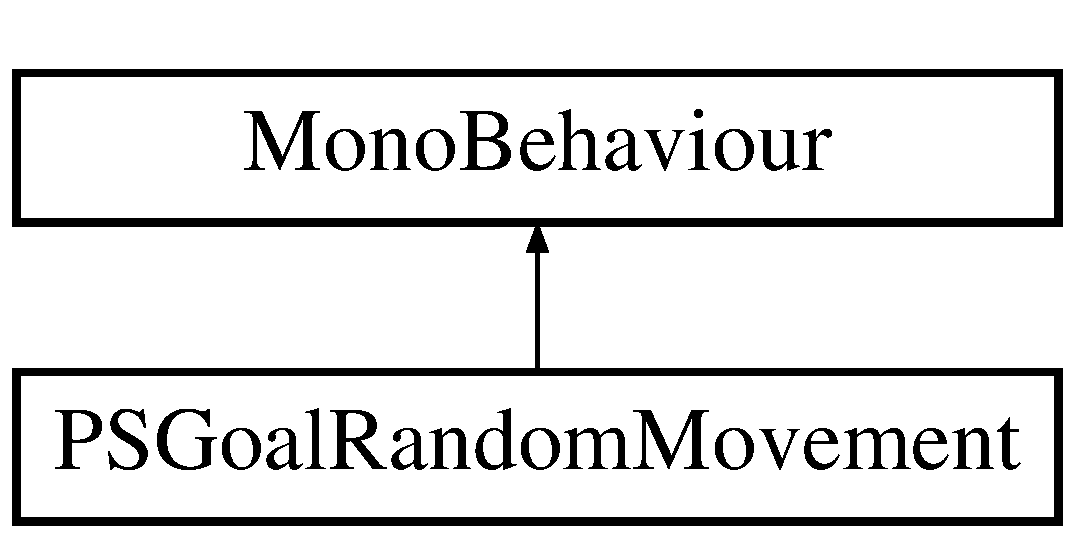
\includegraphics[height=2.000000cm]{class_p_s_goal_random_movement}
\end{center}
\end{figure}
\subsection*{Public Attributes}
\begin{DoxyCompactItemize}
\item 
\mbox{\Hypertarget{class_p_s_goal_random_movement_a15403bed0dac463716ea40bbc9d2db14}\label{class_p_s_goal_random_movement_a15403bed0dac463716ea40bbc9d2db14}} 
float {\bfseries speed} = 1.\+0f
\end{DoxyCompactItemize}


The documentation for this class was generated from the following file\+:\begin{DoxyCompactItemize}
\item 
Assets/\+\_\+\+Scripts/P\+S\+Goal\+Random\+Movement.\+cs\end{DoxyCompactItemize}

\hypertarget{class_p_s_flocking_1_1_p_s_unit_manager}{}\section{P\+S\+Flocking.\+P\+S\+Unit\+Manager Class Reference}
\label{class_p_s_flocking_1_1_p_s_unit_manager}\index{P\+S\+Flocking.\+P\+S\+Unit\+Manager@{P\+S\+Flocking.\+P\+S\+Unit\+Manager}}
Inheritance diagram for P\+S\+Flocking.\+P\+S\+Unit\+Manager\+:\begin{figure}[H]
\begin{center}
\leavevmode
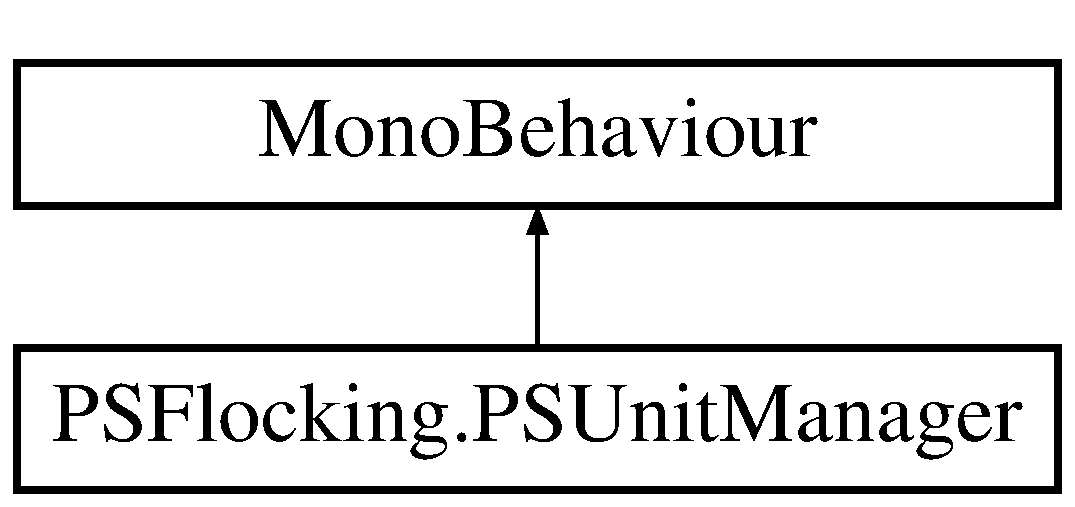
\includegraphics[height=2.000000cm]{class_p_s_flocking_1_1_p_s_unit_manager}
\end{center}
\end{figure}
\subsection*{Public Member Functions}
\begin{DoxyCompactItemize}
\item 
void \hyperlink{class_p_s_flocking_1_1_p_s_unit_manager_a7781ba028d37cfe03fd3c540869751aa}{Add\+Flocking\+Unit} (Game\+Object flocker)
\begin{DoxyCompactList}\small\item\em Adds a unit to the unit list If the passed gameobject does not have a \hyperlink{class_p_s_flocking_1_1_p_s_flocking_unit}{P\+S\+Flocking\+Unit} or a Rigibdoy attached to it, it adds both. The added rigidbody will not use gravity. \end{DoxyCompactList}\item 
void \hyperlink{class_p_s_flocking_1_1_p_s_unit_manager_af7ec7299b52dc9206629f92dcfb601d2}{Remove\+Flocking\+Unit} (Game\+Object flocker)
\begin{DoxyCompactList}\small\item\em Removes a unit from the units-\/list. If the passed unit is not within the unit list, this method does nothing. \end{DoxyCompactList}\end{DoxyCompactItemize}
\subsection*{Public Attributes}
\begin{DoxyCompactItemize}
\item 
\mbox{\Hypertarget{class_p_s_flocking_1_1_p_s_unit_manager_aedaaee6bb56890420722506563f6b588}\label{class_p_s_flocking_1_1_p_s_unit_manager_aedaaee6bb56890420722506563f6b588}} 
List$<$ Game\+Object $>$ \hyperlink{class_p_s_flocking_1_1_p_s_unit_manager_aedaaee6bb56890420722506563f6b588}{units}
\begin{DoxyCompactList}\small\item\em Array holding the units. \end{DoxyCompactList}\item 
\mbox{\Hypertarget{class_p_s_flocking_1_1_p_s_unit_manager_a1a733c51307f36d98644e35d833a7955}\label{class_p_s_flocking_1_1_p_s_unit_manager_a1a733c51307f36d98644e35d833a7955}} 
bool \hyperlink{class_p_s_flocking_1_1_p_s_unit_manager_a1a733c51307f36d98644e35d833a7955}{manual\+Start} = false
\begin{DoxyCompactList}\small\item\em Will not place any units automatically in the scene. \end{DoxyCompactList}\item 
\mbox{\Hypertarget{class_p_s_flocking_1_1_p_s_unit_manager_a4d79206a2784be39d27fcb36c91656e4}\label{class_p_s_flocking_1_1_p_s_unit_manager_a4d79206a2784be39d27fcb36c91656e4}} 
Game\+Object \hyperlink{class_p_s_flocking_1_1_p_s_unit_manager_a4d79206a2784be39d27fcb36c91656e4}{unit\+Prefab}
\begin{DoxyCompactList}\small\item\em Prefab Object from which the units will be created. \end{DoxyCompactList}\item 
\mbox{\Hypertarget{class_p_s_flocking_1_1_p_s_unit_manager_a765240b34b3a5ce19e6f711798c4d1bf}\label{class_p_s_flocking_1_1_p_s_unit_manager_a765240b34b3a5ce19e6f711798c4d1bf}} 
int \hyperlink{class_p_s_flocking_1_1_p_s_unit_manager_a765240b34b3a5ce19e6f711798c4d1bf}{num\+Units} = 100
\begin{DoxyCompactList}\small\item\em Number of units that will be created. \end{DoxyCompactList}\item 
\mbox{\Hypertarget{class_p_s_flocking_1_1_p_s_unit_manager_aa9c3797d524485b906ca919640f80c57}\label{class_p_s_flocking_1_1_p_s_unit_manager_aa9c3797d524485b906ca919640f80c57}} 
Vector3 \hyperlink{class_p_s_flocking_1_1_p_s_unit_manager_aa9c3797d524485b906ca919640f80c57}{spawn\+Range} = new Vector3(10.\+0f, 5f, 10.\+0f)
\begin{DoxyCompactList}\small\item\em The Spawnrange in which the units will be instantiated. \end{DoxyCompactList}\item 
\mbox{\Hypertarget{class_p_s_flocking_1_1_p_s_unit_manager_acab1025d71a518ffd6fdecfbeef80b0a}\label{class_p_s_flocking_1_1_p_s_unit_manager_acab1025d71a518ffd6fdecfbeef80b0a}} 
Game\+Object \hyperlink{class_p_s_flocking_1_1_p_s_unit_manager_acab1025d71a518ffd6fdecfbeef80b0a}{goal}
\begin{DoxyCompactList}\small\item\em A Goal the units will follow, if seek\+Goal is set to true. \end{DoxyCompactList}\item 
\mbox{\Hypertarget{class_p_s_flocking_1_1_p_s_unit_manager_ae308dcd912212ae803fd6d9c48b25288}\label{class_p_s_flocking_1_1_p_s_unit_manager_ae308dcd912212ae803fd6d9c48b25288}} 
bool \hyperlink{class_p_s_flocking_1_1_p_s_unit_manager_ae308dcd912212ae803fd6d9c48b25288}{seek\+Goal} = true
\begin{DoxyCompactList}\small\item\em If set to true, the units will follow the \char`\"{}goal\char`\"{} Game\+Object. \end{DoxyCompactList}\item 
\mbox{\Hypertarget{class_p_s_flocking_1_1_p_s_unit_manager_a6ee39d3bff7f5f98b688738c82dbfbf3}\label{class_p_s_flocking_1_1_p_s_unit_manager_a6ee39d3bff7f5f98b688738c82dbfbf3}} 
bool \hyperlink{class_p_s_flocking_1_1_p_s_unit_manager_a6ee39d3bff7f5f98b688738c82dbfbf3}{obedient} = true
\begin{DoxyCompactList}\small\item\em Will apply random forces to units from time to time, if set to true. \end{DoxyCompactList}\item 
\mbox{\Hypertarget{class_p_s_flocking_1_1_p_s_unit_manager_ad4a71076e0bd500485ef978e3a71ea8e}\label{class_p_s_flocking_1_1_p_s_unit_manager_ad4a71076e0bd500485ef978e3a71ea8e}} 
float \hyperlink{class_p_s_flocking_1_1_p_s_unit_manager_ad4a71076e0bd500485ef978e3a71ea8e}{max\+Force} = 4.\+0f
\begin{DoxyCompactList}\small\item\em The maximum Force that will be applied to the units. \end{DoxyCompactList}\item 
\mbox{\Hypertarget{class_p_s_flocking_1_1_p_s_unit_manager_a5c4bed8aa8fd71ce724c813e0903e0fb}\label{class_p_s_flocking_1_1_p_s_unit_manager_a5c4bed8aa8fd71ce724c813e0903e0fb}} 
float \hyperlink{class_p_s_flocking_1_1_p_s_unit_manager_a5c4bed8aa8fd71ce724c813e0903e0fb}{maxvelocity} = 2.\+0f
\begin{DoxyCompactList}\small\item\em The maximum Velocity the units can reach. \end{DoxyCompactList}\item 
\mbox{\Hypertarget{class_p_s_flocking_1_1_p_s_unit_manager_a4bced9fa2de0369f6288e5d65cb0fc4b}\label{class_p_s_flocking_1_1_p_s_unit_manager_a4bced9fa2de0369f6288e5d65cb0fc4b}} 
float \hyperlink{class_p_s_flocking_1_1_p_s_unit_manager_a4bced9fa2de0369f6288e5d65cb0fc4b}{alignment\+Strength} = 0.\+5f
\begin{DoxyCompactList}\small\item\em Sets how much the units will align to each other. \end{DoxyCompactList}\item 
\mbox{\Hypertarget{class_p_s_flocking_1_1_p_s_unit_manager_aa45a0fe01bcf38a17e9e9f315455a820}\label{class_p_s_flocking_1_1_p_s_unit_manager_aa45a0fe01bcf38a17e9e9f315455a820}} 
float \hyperlink{class_p_s_flocking_1_1_p_s_unit_manager_aa45a0fe01bcf38a17e9e9f315455a820}{alignment\+Distance} = 6
\begin{DoxyCompactList}\small\item\em The maximum distance that units can be away from each other to make alignmet work. \end{DoxyCompactList}\item 
\mbox{\Hypertarget{class_p_s_flocking_1_1_p_s_unit_manager_a86b7428c21b9f76a78dd13221c4ff700}\label{class_p_s_flocking_1_1_p_s_unit_manager_a86b7428c21b9f76a78dd13221c4ff700}} 
float \hyperlink{class_p_s_flocking_1_1_p_s_unit_manager_a86b7428c21b9f76a78dd13221c4ff700}{cohesion\+Strength} = 0.\+5f
\begin{DoxyCompactList}\small\item\em Sets how much the units will stick to each other. \end{DoxyCompactList}\item 
\mbox{\Hypertarget{class_p_s_flocking_1_1_p_s_unit_manager_a9ffaea9774cccd08c81b501dd6965fac}\label{class_p_s_flocking_1_1_p_s_unit_manager_a9ffaea9774cccd08c81b501dd6965fac}} 
float \hyperlink{class_p_s_flocking_1_1_p_s_unit_manager_a9ffaea9774cccd08c81b501dd6965fac}{cohesion\+Distance} = 6
\begin{DoxyCompactList}\small\item\em The maximum distance that units can be away from each other to make cohesion work. \end{DoxyCompactList}\item 
\mbox{\Hypertarget{class_p_s_flocking_1_1_p_s_unit_manager_aa24cb0b36be539ede2aafc43952f4f03}\label{class_p_s_flocking_1_1_p_s_unit_manager_aa24cb0b36be539ede2aafc43952f4f03}} 
float \hyperlink{class_p_s_flocking_1_1_p_s_unit_manager_aa24cb0b36be539ede2aafc43952f4f03}{separation\+Strength} = 0.\+5f
\begin{DoxyCompactList}\small\item\em Sets how much the units will try to move away from each other. \end{DoxyCompactList}\item 
\mbox{\Hypertarget{class_p_s_flocking_1_1_p_s_unit_manager_a8d462943657ab150dc43d8007e8d52d0}\label{class_p_s_flocking_1_1_p_s_unit_manager_a8d462943657ab150dc43d8007e8d52d0}} 
float \hyperlink{class_p_s_flocking_1_1_p_s_unit_manager_a8d462943657ab150dc43d8007e8d52d0}{separation\+Distance} = 5
\begin{DoxyCompactList}\small\item\em The maximum distance that units can be away from each other to make separation work. \end{DoxyCompactList}\item 
\mbox{\Hypertarget{class_p_s_flocking_1_1_p_s_unit_manager_a7d2b62844ac4629ec9d6d90327741768}\label{class_p_s_flocking_1_1_p_s_unit_manager_a7d2b62844ac4629ec9d6d90327741768}} 
float \hyperlink{class_p_s_flocking_1_1_p_s_unit_manager_a7d2b62844ac4629ec9d6d90327741768}{randomizer\+Strength} = 0.\+2f
\begin{DoxyCompactList}\small\item\em Sets how much randomized Force should be applied to the units. \end{DoxyCompactList}\item 
\mbox{\Hypertarget{class_p_s_flocking_1_1_p_s_unit_manager_a8b2bb3c41213b2298582fa2f195e394a}\label{class_p_s_flocking_1_1_p_s_unit_manager_a8b2bb3c41213b2298582fa2f195e394a}} 
float \hyperlink{class_p_s_flocking_1_1_p_s_unit_manager_a8b2bb3c41213b2298582fa2f195e394a}{viewing\+Angle} = 170.\+0f
\begin{DoxyCompactList}\small\item\em The angle in which a Boid can \char`\"{}see\char`\"{} others. Cohesion, Alignment, Separation will only be applied if units are within the viewing Angle. \end{DoxyCompactList}\end{DoxyCompactItemize}
\subsection*{Protected Member Functions}
\begin{DoxyCompactItemize}
\item 
\mbox{\Hypertarget{class_p_s_flocking_1_1_p_s_unit_manager_a5ddc6c91220d066b472093428b21ee2b}\label{class_p_s_flocking_1_1_p_s_unit_manager_a5ddc6c91220d066b472093428b21ee2b}} 
void \hyperlink{class_p_s_flocking_1_1_p_s_unit_manager_a5ddc6c91220d066b472093428b21ee2b}{Start} ()
\begin{DoxyCompactList}\small\item\em Called once from Unity. Do not call manually. Sets up the units and places them at a random position within the Spawn\+Range. \end{DoxyCompactList}\end{DoxyCompactItemize}


\subsection{Detailed Description}
The manager that holds a list of all units, and all attributes about the flock. 

\subsection{Member Function Documentation}
\mbox{\Hypertarget{class_p_s_flocking_1_1_p_s_unit_manager_a7781ba028d37cfe03fd3c540869751aa}\label{class_p_s_flocking_1_1_p_s_unit_manager_a7781ba028d37cfe03fd3c540869751aa}} 
\index{P\+S\+Flocking\+::\+P\+S\+Unit\+Manager@{P\+S\+Flocking\+::\+P\+S\+Unit\+Manager}!Add\+Flocking\+Unit@{Add\+Flocking\+Unit}}
\index{Add\+Flocking\+Unit@{Add\+Flocking\+Unit}!P\+S\+Flocking\+::\+P\+S\+Unit\+Manager@{P\+S\+Flocking\+::\+P\+S\+Unit\+Manager}}
\subsubsection{\texorpdfstring{Add\+Flocking\+Unit()}{AddFlockingUnit()}}
{\footnotesize\ttfamily void P\+S\+Flocking.\+P\+S\+Unit\+Manager.\+Add\+Flocking\+Unit (\begin{DoxyParamCaption}\item[{Game\+Object}]{flocker }\end{DoxyParamCaption})}



Adds a unit to the unit list If the passed gameobject does not have a \hyperlink{class_p_s_flocking_1_1_p_s_flocking_unit}{P\+S\+Flocking\+Unit} or a Rigibdoy attached to it, it adds both. The added rigidbody will not use gravity. 


\begin{DoxyParams}{Parameters}
{\em flocker} & Game\+Object that should be added to the units list. \\
\hline
\end{DoxyParams}
\mbox{\Hypertarget{class_p_s_flocking_1_1_p_s_unit_manager_af7ec7299b52dc9206629f92dcfb601d2}\label{class_p_s_flocking_1_1_p_s_unit_manager_af7ec7299b52dc9206629f92dcfb601d2}} 
\index{P\+S\+Flocking\+::\+P\+S\+Unit\+Manager@{P\+S\+Flocking\+::\+P\+S\+Unit\+Manager}!Remove\+Flocking\+Unit@{Remove\+Flocking\+Unit}}
\index{Remove\+Flocking\+Unit@{Remove\+Flocking\+Unit}!P\+S\+Flocking\+::\+P\+S\+Unit\+Manager@{P\+S\+Flocking\+::\+P\+S\+Unit\+Manager}}
\subsubsection{\texorpdfstring{Remove\+Flocking\+Unit()}{RemoveFlockingUnit()}}
{\footnotesize\ttfamily void P\+S\+Flocking.\+P\+S\+Unit\+Manager.\+Remove\+Flocking\+Unit (\begin{DoxyParamCaption}\item[{Game\+Object}]{flocker }\end{DoxyParamCaption})}



Removes a unit from the units-\/list. If the passed unit is not within the unit list, this method does nothing. 


\begin{DoxyParams}{Parameters}
{\em flocker} & Game\+Object that shold be removed from the units list. \\
\hline
\end{DoxyParams}


The documentation for this class was generated from the following file\+:\begin{DoxyCompactItemize}
\item 
Assets/\+\_\+\+Scripts/P\+S\+Unit\+Manager.\+cs\end{DoxyCompactItemize}

%--- End generated contents ---

% Index
\backmatter
\newpage
\phantomsection
\clearemptydoublepage
\addcontentsline{toc}{chapter}{Index}
\printindex

\end{document}
